% \chapter{КХЭД как сеть массового обслуживания} \label{chapt3}
\subsection{КХЭД как сеть массового обслуживания} \label{net}
% \addcontentsline{toc}{chapter}{КХЭД как сеть массового обслуживания}  % Добавляем его в оглавление

\textbf{\textit{Система массового обслуживания (СМО)}} -- система, производящая обслуживание поступающих в неё требований. \textbf{\textit{Заявки}} (требования) поступают от нескольких источников через постоянные или произвольные промежутки времени. \textbf{\textit{Приборы}} (каналы) служат для обработки этих заявок. Если в момент поступления заявки все приборы заняты, заявка поступает в \textbf{\textit{очередь}} на обслуживание. Очередь может быть конечной или бесконечной. В случае переполнения конечной очереди заявка получает \textbf{\textit{отказ}} с вероятностью, называемой \textbf{\textit{вероятностью потери заявки}}.

\vspace{\baselineskip}
Для обозначения типа СМО Кендаллом и Башариным предложена система обозначений, имеющих вид $\Delta / \Theta / \Xi / \Omega$. \cite{bib4,bib5,bib6} Здесь $\Delta$ -- обозначение закона распределения вероятностей для интервалов поступления заявок, $\Theta$ – обозначение закона распределения вероятностей для времени, $\Xi$ – число каналов обслуживания, $\Omega$ – число мест в очереди.

\vspace{\baselineskip}
Обозначение законов распределения в позициях $\Delta$ и $\Theta$ выполняется обычно буквами из следующего списка:

\begin{itemize}
  \item $M$ -- экспоненциальное,
  \item $E^k$ -- эрланговское порядка $k$,
  \item $R$ -- равномерное,
  \item $D$ -- детерминированное (постоянная величина),
  \item $G$ -- произвольное (любого вида).
\end{itemize}

Если число мест в очереди не ограничено, то позиция $\Xi$ не указывается.
Например, $M/M/1$ означает простейшую СМО (оба распределения экспоненциальные, канал обслуживания один, очередь не ограничена), а обозначение $R/D/2/100$ соответствует СМО с равномерным распределением интервалов поступления требований, фиксированным временем их обслуживания, двумя каналами и 100 местами в очереди. В этой СМО заявки, приходящие в моменты, когда все места в очереди заняты, покидают систему (т.е. теряются).

\vspace{\baselineskip}
\textbf{\textit{Сеть массового обслуживания (СеМО)}} -- совокупность конечного числа обслуживающих узлов, в которой циркулируют заявки, переходящие в соответствии с маршрутной матрицей из одного узла в другой. Узел всегда является разомкнутой СМО, т.е. имеющей входящий и исходящий поток сообщений (заявок).

\vspace{\baselineskip}
В соответствии с теорией массового обслуживания, можно классифицировать КХЭД как разомкнутую экспоненциальную сеть массового обслуживания. \cite{bib3} Для таких СеМО равновесное совместное распределение количества заявок в центрах обслуживания представляется в виде произведения маргинальных распределений:
\begin{equation}
  \label{eq:equation1}
  P(n_1,n_2,\ldots,n_k) = \prod_{i=1}^R P_i(n_i),
\end{equation}
где $P_i(n_i)$ -- стационарная вероятность того, что в $i$-м центре, рассматриваемом изолированно, находится  $n_i$ сообщений, $R$ -- количество центров массового обслуживания в сети.

\vspace{\baselineskip}
Для определения потоков, циркулирующих в стационарном режиме в сети МО, вводятся коэффициенты передачи  $e_i$, такие, что $\lambda(N)e_i$ представляет собой общую интенсивность потока сообщений в $i$-й центр сети $(i=\overline{1,R})$, $\lambda(N)$ -- интенсивность входящего в СеМО потока сообщений:
$$
\lambda_i(N)=\lambda(N)e_i, i=\overline{1,R}.
$$

В открытых СеМО интенсивность  $\lambda_i$ складывается из интенсивности поступления сообщений в $i$-й центр из источника и интенсивности поступления из других центров:
\begin{equation}
  \label{eq:equation2}
e_i = P_{oi} + \sum_{j=1}^R P_{ij}e_j, i=\overline{1,R}.
\end{equation}

В случае замкнутых сетей исключается поток от внешнего источника. Для отыскания однозначного решения системы уравнений (\ref{eq:equation2}) достаточно произвольно задать значение $e_i$, например, положить $e_i=1$. В этом случае величину $e_i$ можно интерпретировать как среднее число посещений центра $i$ между двумя последовательными посещениями первого центра.

\vspace{\baselineskip}
На рис. \ref{img:net} представлена формализованная схема КХЭД в виде СеМО.

% \begin{figure} [h] 
%   \center
%   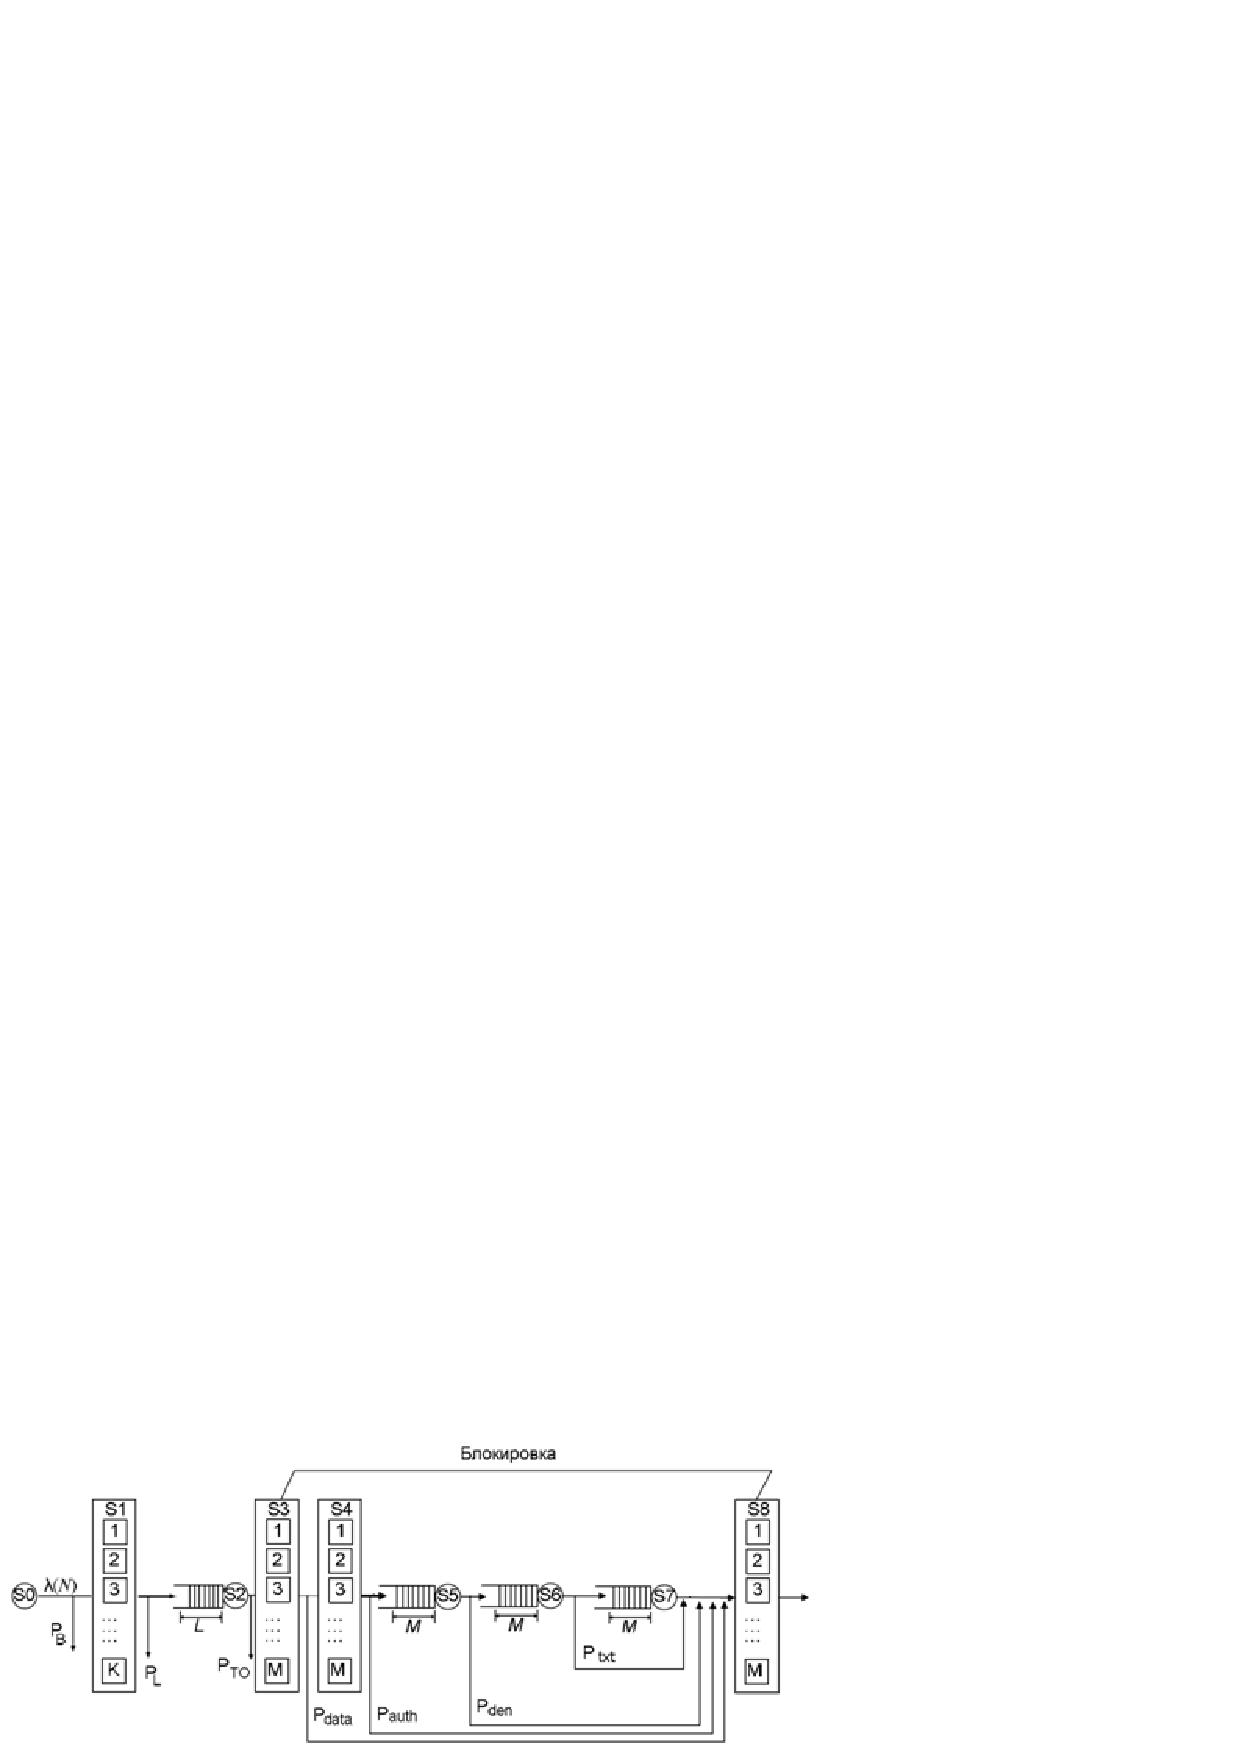
\includegraphics [scale=0.9] {net.jpg}
%   \caption{Открытая сеть массового обслуживания, формализующая работу КХЭД} 
%   \label{img:net}  
% \end{figure}
\begin{figure}[h]
  \centering
  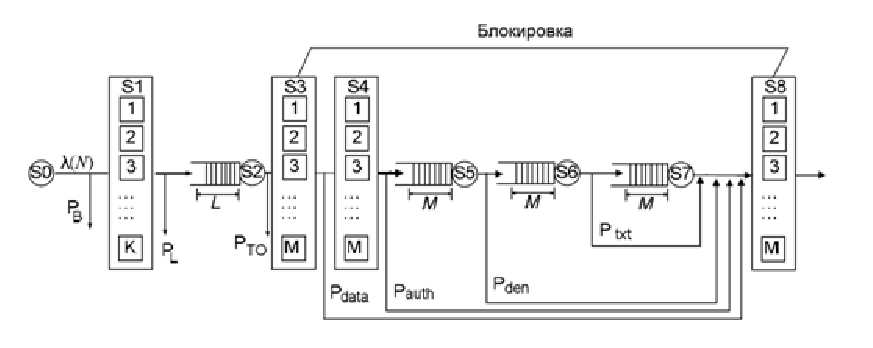
\includegraphics[width=1\textwidth]{net}
  \caption{Открытая сеть массового обслуживания, формализующая работу КХЭД}
  \label{img:net}
\end{figure}

% \vspace{\baselineskip}
$S0$ -- центр, формализующий входной поток сообщений пользователей.

\vspace{\baselineskip}
$S1$ -- центр, формализующий работу модуля TCP (транспортный уровень) операционной системы сервера приложений КХЭД на этапе установления соединения. $K$ – число обслуживающих каналов, очередь отсутствует. Если в момент поступления сообщения в центр все $K$ каналов заняты, то сообщение теряется, вероятность этого события равна $P_B$.

\vspace{\baselineskip}
$S2$ -- основной поток приложения сервера, извлекающего сообщения из очереди на установление соединения. Максимальная длина очереди $L$ к центру задается в серверном приложении. Если при поступлении сообщения все $L$ мест очереди заняты, то сообщение теряется с вероятностью $P_L$.

\vspace{\baselineskip}
$S3$ -- параллельные потоки сервера, обеспечивающие одновременное обслуживание соединений на этапе получения запросов по сети. При переполнении центра сообщения теряются с вероятностью $P_{TO}$.
Центры $S1$, $S2$, $S3$ реализуют \underline{модуль установки соединения}.

\vspace{\baselineskip}
Центры $S3$ и $S8$ имеют по $M$ каналов обслуживания (потоков сервера) и при начале обслуживания сообщения в $i$-ом канале центра $S3$ он считается занятым до завершения обслуживания в $i$-ом канале центра $S8$. Таким образом, происходит блокировка каналов центров $S3$ и $S8$ и поэтому потерь сообщений из-за переполнения очереди к центрам $S5$, $S6$, $S7$ и занятости всех обслуживающих устройств центра $S4$ не происходит, т.к. больше чем $M$ сообщений в центрах $S4$, $S5$, $S6$, $S7$ быть не может.

\vspace{\baselineskip}
$S4$ -- \underline{модуль аутентификации} клиентов при обращении к КХЭД.

\vspace{\baselineskip}
$S5$ -- \underline{модуль проверки прав доступа} клиентов при обращении к КХЭД.

\vspace{\baselineskip}
В случае удачной аутентификации и проверки прав доступа клиента производится поиск электронного документа по запросу пользователя и выполнение операций по контролю целостности информации, проверке и простановки ЭЦП, шифрованию и дешифрованию. Для формализации процесса поиска и редактирования электронных документов выделены центры $S6$ и $S7$ соответственно.
После того, как запрос пользователя выполнен, происходит передача ответа пользователю в многолинейном центре обслуживания $S8$.

\vspace{\baselineskip}
В соответствии с теоремой BCMP (Baskett, Chandy, Muntz, Palacios) мультипликативное свойство решения (\ref{eq:equation1}) для $P_(n_1,n_2,\ldots,n_R)$ сохраняется для СеМО, содержащих следующие виды узлов:
\begin{itemize}
  \item $M/M/m$ с дисциплиной обслуживания FCFS (First Came First Served -- первым поступил, первым обслужен);
  \item $M/G/1$ с дисциплиной дисциплиной PS (Process Sharing -- разделение процессора);
  \item $M/G/\infty$ с обслуживанием без ожидания (IS -- Immediately Serve);
  \item $M/G/1$ с дисциплиной LCFS (Last Came First Served -- последним поступил, первым обслужен) с прерываниями.\cite{bib7}
\end{itemize}

% \vspace{\baselineskip}
В приведённой на рис. \ref{img:net} схеме представлены следующие узлы:
\begin{itemize}
  \item $S1, S3, S4, S8 - M/G/\infty$, IS;
  \item $S2, S6, S7 - M/M/1$, FCFS;
  \item $S5 - M/G/1$, PS.\cite{bib3}
\end{itemize}

% \vspace{\baselineskip}
Одной из важнейших задач СЭД является обнаружение ошибок редактора. Такие ошибки делятся соответственно на \textit{детектируемые} и \textit{недетектируемые}.
Описанная на рис. \ref{img:net} СеМО обнаруживает следующие типы ошибок:
\begin{itemize}
  \item Неверное предоставление аутентификационных данных -- эта ошибка появляется с вероятностью $P_{data}$;
  \item Отсутствие прав доступа к запрашиваемому документу -- с вероятностью $P_{auth}$;
  \item Ошибка поиска -- с вероятностью $P_{den}$;
  \item Ошибки во вносимых изменениях (напр., обращение к некорректным полям документа) -- с вероятностью $P_{txt}$.
\end{itemize}

% \vspace{\baselineskip}
Механизм обнаружения таких ошибок позволяет избежать выдачи заведомо неверного документа следующему редактору в схеме, представленной на рис. \ref{img:graph1}.

\vspace{\baselineskip}
С учётом вышеописанного, каждый из редакторов в схеме на рис. \ref{img:graph1} может быть представлен в виде автоматизированной системы, изображённой на рис. \ref{img:as}.

\begin{figure}[h]
  \centering
  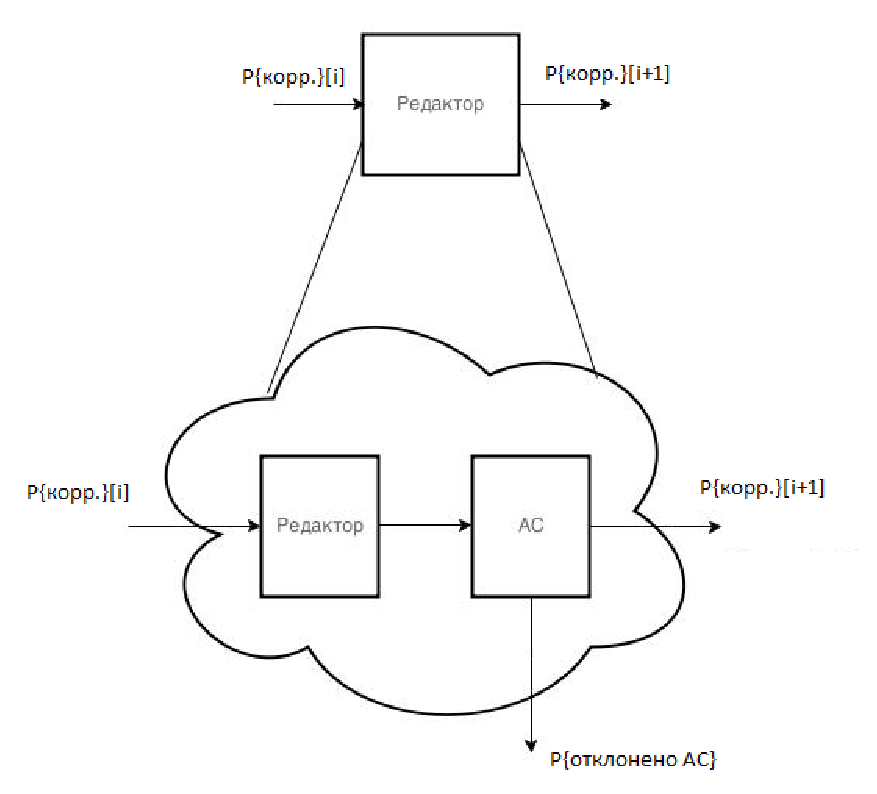
\includegraphics[width=0.6\textwidth]{as}
  \caption{Схема узла СЭД с применением АС для обработки данных}
  \label{img:as}
\end{figure}

В роли АС здесь выступает КХЭД, описанное на рис. \ref{img:net}. В случае обнаружения ошибок силами АС пользователю выдаётся сообщение об ошибке, т.е. фактически новое задание на редактирование. С учётом этого факта граф, представленный на рис. \ref{img:graph1}, преобразуется к виду:

\begin{figure}[h]
  \centering
  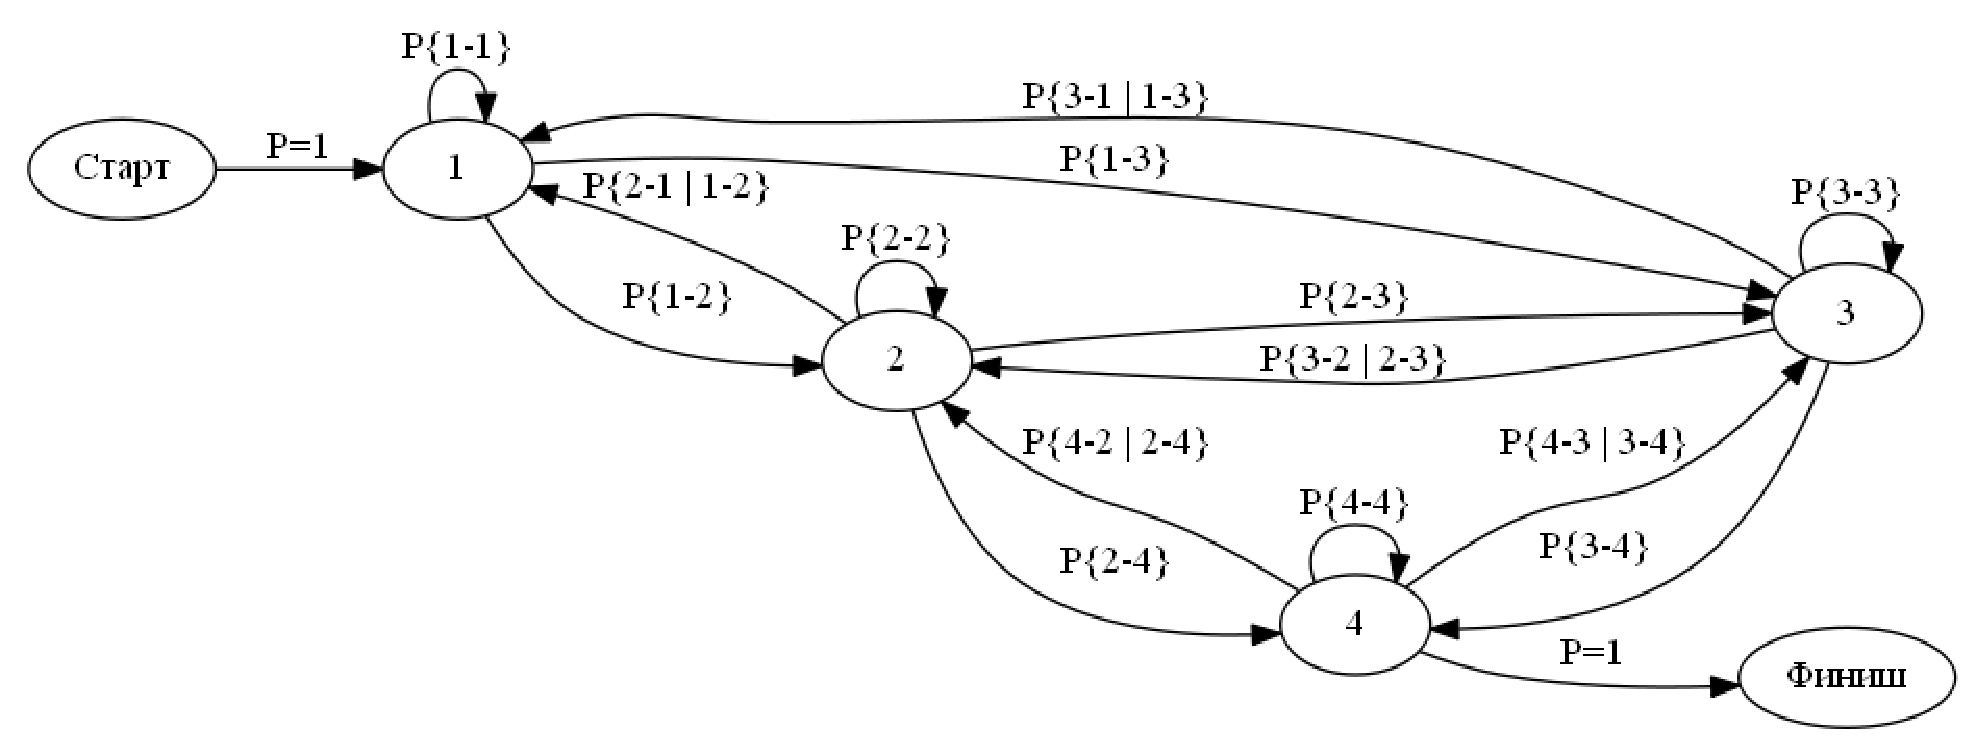
\includegraphics[width=1\textwidth]{graph2}
  \caption{Документооборот с применением СЭД}
  \label{img:graph2}
\end{figure}

% \clearpage